\begin{figure}[htbp]
  \centering
  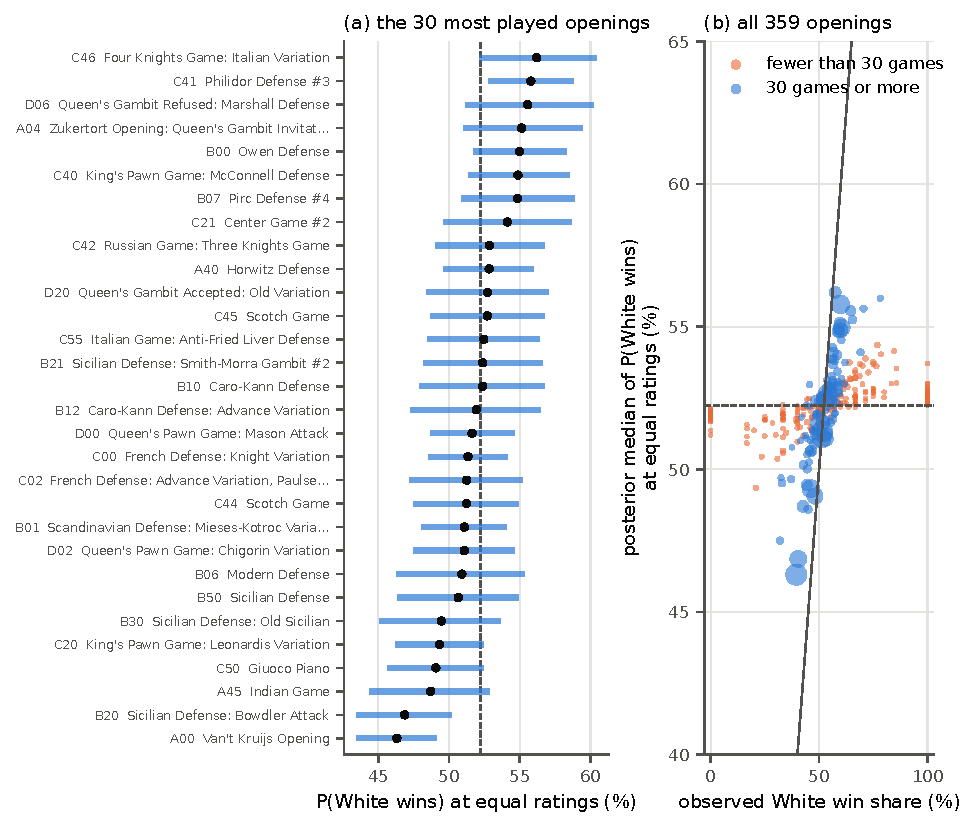
\includegraphics[width=\linewidth]{openings.pdf}
  \caption{Effect of the opening on White's chance of winning. (a): posterior median and central 90\% interval of $\operatorname{logit}^{-1}(\theta_o)$, the probability that White wins when both players have the same rating, for the 30 openings with the most games, ordered by posterior median. The dashed line is the average opening, $\operatorname{logit}^{-1}(\mu)$, at 52.2\%. Each label is an ECO code with the most frequent opening name among its games; one ECO code groups several variations. The 90\% interval lies entirely above the average for 1 of these 30 openings and entirely below it for 2; the others cannot be told apart from the average opening. (b): observed White win share of every opening against its posterior median, with the area of each point proportional to the number of games, the identity line in gray and the dashed line the average opening. Openings with few games are pulled almost all the way to the average, and openings with many games stay near their observed share; the remaining gap from the identity line also reflects the rating gaps of the games, which the model accounts for and the observed share does not.}
  \label{fig:openings}
\end{figure}
